\section{Implementation}
\label{sec:implementation}

\begin{figure}[t]
\begin{centering}
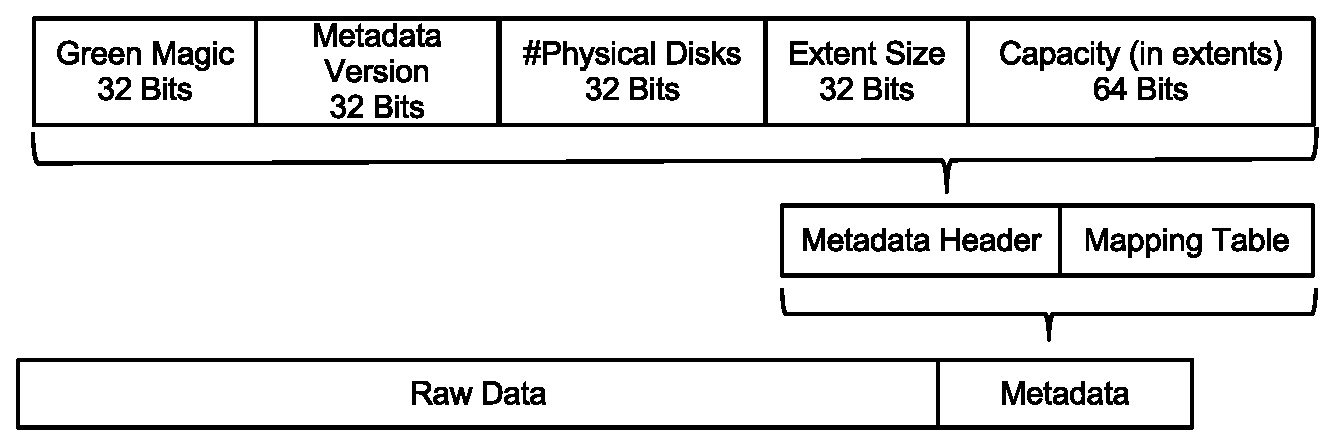
\epsfig{file=figures/metadata.eps,width=1.00\linewidth}
\caption{Metadata of green device on a disk. Metadata is placed at the
end of raw data, and it has a replica on each physical disk.}
\label{fig:metadata}
\end{centering}
\end{figure}


We implemented our multi-disk driver as a Linux Device Mapper target.
Figure \ref{fig:metadata} showes the metadata organization of a green
device. Figure \ref{fig:rwpath} presents the pesudocode of the BIO
redirection. When there is no need for extent migration, our target
simply looks up into the mapping table and maps BIOs accordingly.
Migration of extents are implemented using either \texttt{dm\_io}
(migration not divided) or \texttt{dm\_kcopyd} (migration divided into
promotion and demotion).  Both of them are infrastructure services of
the Device Mapper framework.  \texttt{dm\_io} is used for performing
disk I/O and it can be synchronous (if set callback function to null)
or asynchronous (if callback function is not null).
\texttt{dm\_kcopyd} provides asynchronous data copying between disks. 

\begin{figure}[t]
{\footnotesize 
\begin{verbatim}
int green_map(bio) {
  ext_id = bio->offset / ext_size;
  if (ext_id does not have mapping) {
    if (there is space on cache disk) {
      physical_ext = get_ext_from_cache();
    } else {
      physical_ext = get_ext_from_secondary();
    }
    table[ext_id] = physical_ext;
  } 
  physical_ext = table[ext_id];
  if (physical_ext on cache and bio is Read) {
    schedule_ext_migration(physical_ext);
    return DM_MAPIO_SUBMITTED;
  } 
  map_bio_to_physical_device(bio, physical_ext);
  return DM_MAPIO_REMAPPED;
}
\end{verbatim}
}
\caption{Pesudocode of the BIO redirection.} 
\label{fig:rwpath}
\end{figure}


Because extent migration involves at least two I/Os (one read and one
write), it is slow and not atomic. It is slow, so we limited the
maximum number of concurrent migration. Otherwise, there can be too
many migrations that the I/O performance degrades severely under heavy
IO load. For example, when the whole disk is scanned
multiple times, the SSD will thrash because of the LRU heuristic. It
is not atomic, so we have to suspend the BIOs targeting those extents that
are under migration. We kept a queue of BIOs for every migrating
extent and we submit all the BIOs once migrating is done (no matter on
success or failure). To achieve good throughput, we do not wait for
migration to finish before continue to map more BIOs. We queued all
migrations and returns immediately. A daemon, implemented using Linux
\texttt{workqueue}, schedules them later.

Because I/O schedulers reorder I/O requests to maximize throughput,
BIOs are not served in the same order as we submit them to underlying
disks.  When we access an extent, it is possible that the extent to 
which I/O request is raised gets migrated between the time we submit the request and the
time the request is served. In this case, we end up getting wrong
data.  To avoid this, we have to make sure all requests of an extent
are finished before we migrate it. We associated an atomic counter
with each extent. The counter is incremented before we send a request
to the corresponding extent, and it is decremented after the request
is finished. Then migration only occurs for those extents whose
counters are zero.  (This part code is not finished). 

We have written a userland program which accepts signal (with major
and minor device number) from our target and invokes \texttt{hdparm}
to put disks into low-power states.  There are two low-power states,
which are standby (spin down) and sleeping (power down).
\texttt{hdparm} can achieve both of them  as long as the disks has
these features. There are also two ways to put disks into low-power
states. One is to set a timeout and disks are put into low-power
states when they are idle for that long time. Another is to spin/power
down disks at once. We do not have to spin/power up in our code
because disks go up once they are accessed. 

%%%%%%%%%%%%%%%%%%%%%%%%%%%%%%%%%%%%%%%%%%%%%%%%%%%%%%%%%%%%%%%%%%%%%%%%%%%%%%
%% For Emacs:
% Local variables:
% fill-column: 70
% End:
%%%%%%%%%%%%%%%%%%%%%%%%%%%%%%%%%%%%%%%%%%%%%%%%%%%%%%%%%%%%%%%%%%%%%%%%%%%%%%
%% For Vim:
% vim:textwidth=70
%%%%%%%%%%%%%%%%%%%%%%%%%%%%%%%%%%%%%%%%%%%%%%%%%%%%%%%%%%%%%%%%%%%%%%%%%%%%%%
% LocalWords:  SMR HDDs drive's SMRs
